\section{Evaluation of Interest flooding mitigation methods}
\label{sec:evaluation}

\todo{Both simulation, as well as emulation for various sized topologies (trees as well as real topologies), various parameters etc.
List all possible parameters, say clearly which ones we vary, and which ones we do not, along with explanations.

Metrics that we will consider in our evaluation (Satisfaction rate for good clients, Link utilization near producers, Latency for good clients, good versus bad interests as a function of time).}

We want to explore the effectiveness of designed mitigation techniques in a two distinctive ways. First, we need to understand how each method works on a very ground level of a just few nodes and links. Second, we want to pick promising techniques and see if they work in a large scale networks of hundreds and thousands of nodes. To ensure the correct transition from small scale experiments to large scale experiments we had to use the same evaluation tool in order to eliminate any possibility of implementation discrepancy. As of today the only network simulator supporting full NDN logic is the NS-3 based ndnSIM software. 

\subsection{Small-scale evaluations}
\label{sec:small-scale}

\begin{figure}[htbp]
  \centering
  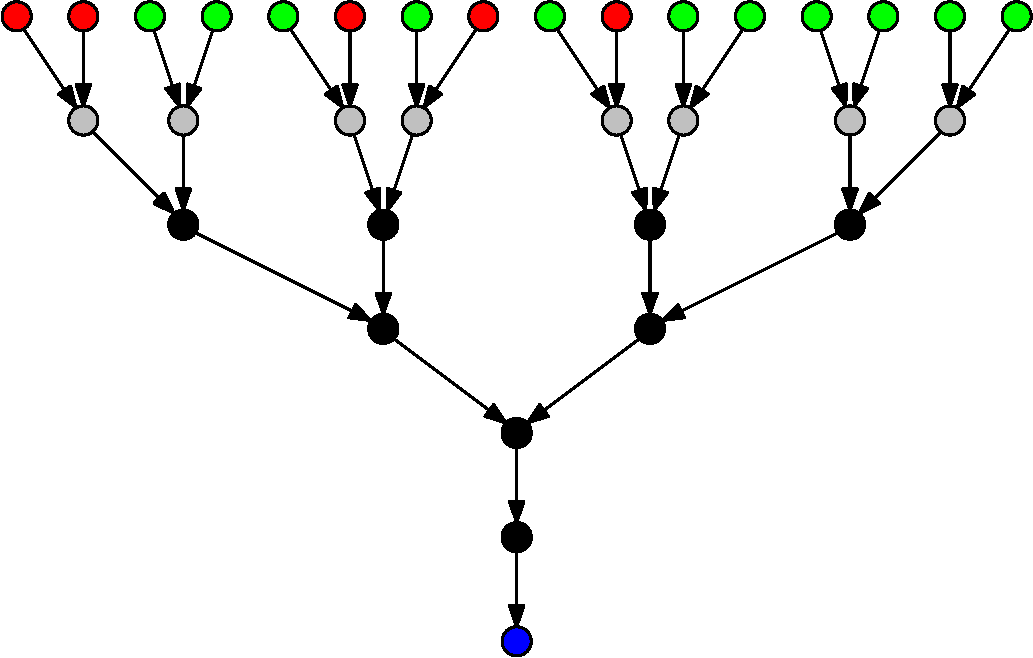
\includegraphics[scale=0.3]{topo-tree-evil-5-good-0-producer-gw}
  \caption{Small-scale topology (one of the runs with 30\% of attackers, all links are 10Mbps with randomized delay 1-10ms)}
  \label{fig:small-scale-topo}
\end{figure}


\begin{figure}[htbp]
  \centering
  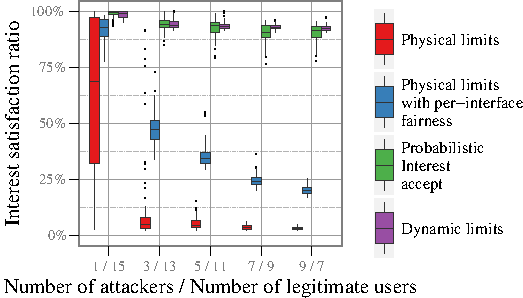
\includegraphics[scale=1]{tree-topo-var-evils-max-consumers-30mins/tree-good-0-producer-gw-avg-1-min}
  \caption{Average consumer Interest satisfaction ratios (first minute)}
  \label{fig:small-scale-topo 1}
\end{figure}


\begin{figure}[htbp]
  \centering
  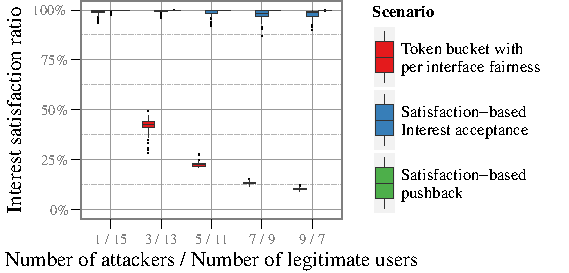
\includegraphics[scale=1]{tree-topo-var-evils-max-consumers-30mins/tree-good-0-producer-gw-avg-1-min-after-1-min}
  \caption{Average consumer Interest satisfaction ratios (second minute)}
  \label{fig:small-scale-topo 2}
\end{figure}

\begin{figure}[htbp]
  \centering
  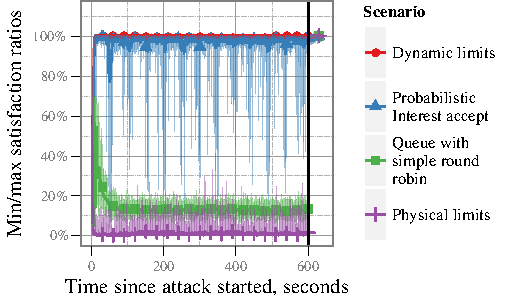
\includegraphics[scale=1]{tree-topo-var-evils-max-consumers-30mins/tree-good-0-producer-gw-dynamics-40}
  \caption{Satisfaction ratio dynamics during the attack (7 attackers / 9 legitimate)}
  \label{fig:small-scale-topo 3}
\end{figure}


%%% Local Variables: 
%%% mode: latex
%%% TeX-master: "paper"
%%% End: 

\subsection{Large scale simulations}
\label{sec:largescale}

Large scale, large scale

%\begin{figure}[htpb]
%  \centering
%  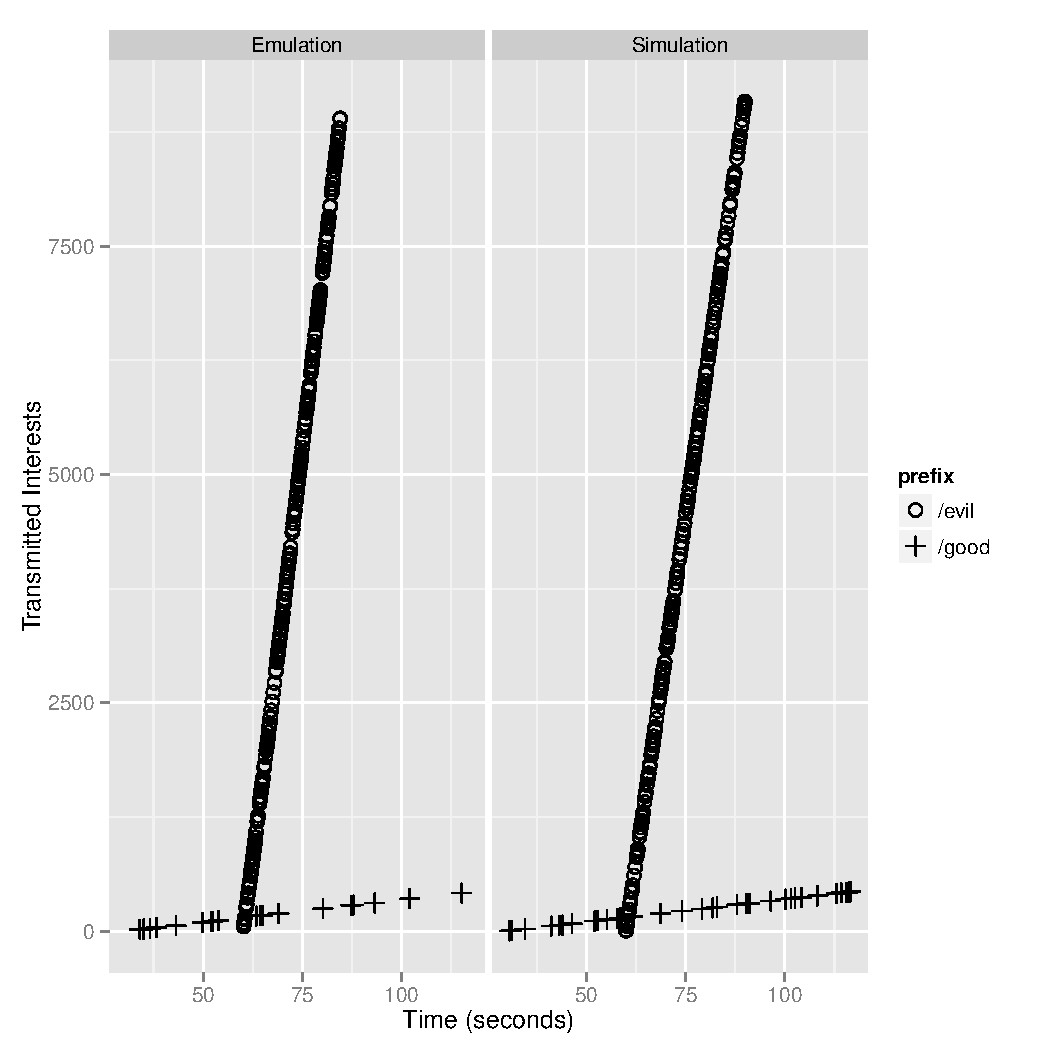
\includegraphics[scale=0.5]{figures/sim-emu-power.pdf}
%  \caption{Strength of Interest flooding attack}
%  \label{fig:simemupower}
%\end{figure}

%\begin{figure}[htpb]
%  \centering
%  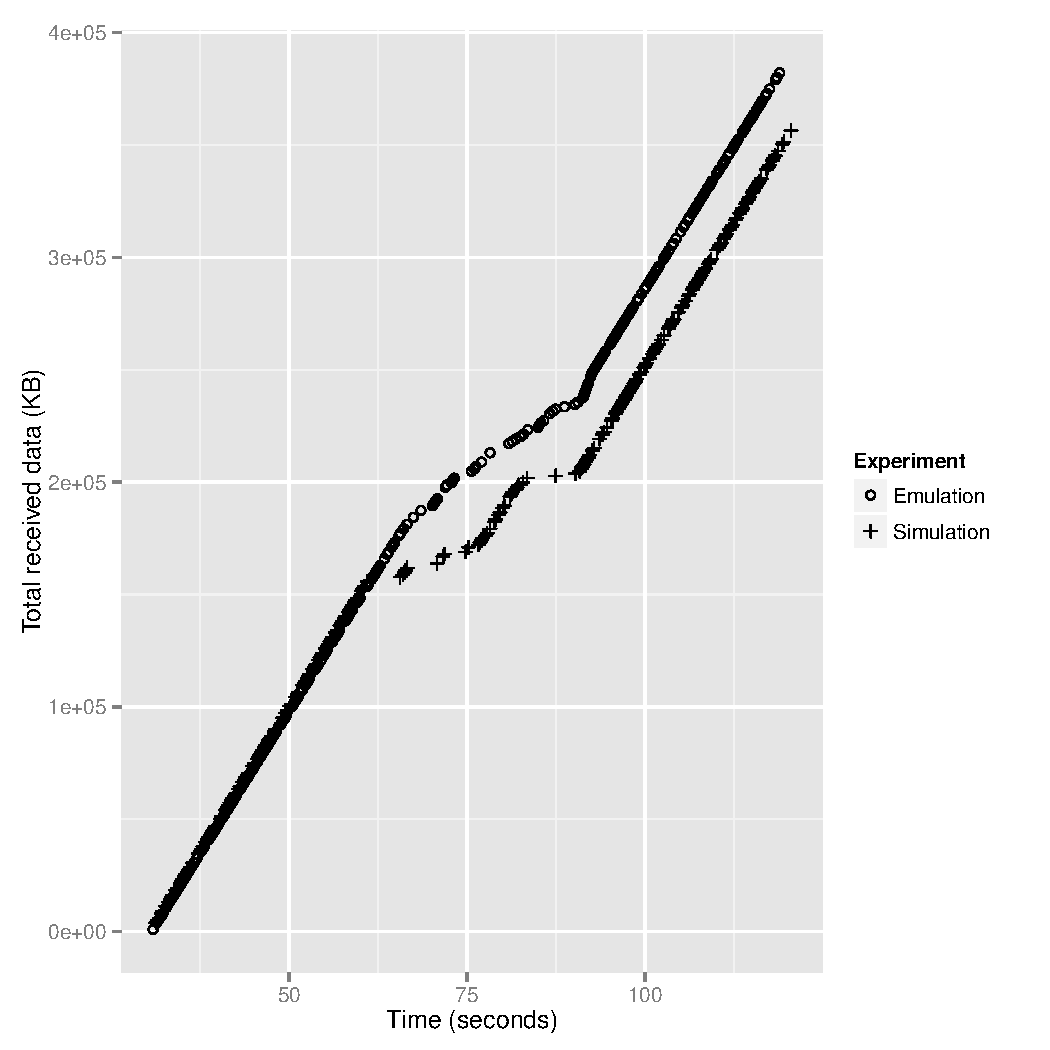
\includegraphics[scale=0.5]{figures/sim-emu-performance.pdf}
%  \caption{Data retrieval by legitimate clients}
%  \label{fig:simemuperf}
%\end{figure}



% \subsection{Simulation versus Emulation}
\label{sec:simemu}
Before committing significant efforts into simulation-based implementation of designed defensive techniques it was necessary to confirm that ndnSIM has close performance characteristics to the reference NDN implementation - Project CCNx. This will guarantee that evaluation results derived from simulations will be meaningful in real NDN world.

To achieve this goal a comparison of Project CCNx software and ndnSIM software was performed under small scale Interest flooding attack. DETER Testbed was used as emulation tool for CCNx evaluation. Using it we were able to setup non-virtualized Ubuntu nodes running CCNx 0.6.0 software connected in a binary tree topology with 4 leaves and 1 root node. A number of applications running on top of CCNx have been developed, namely:
\begin{itemize}
\item{Producer application serves 1KB data packets under a known for the attacker name prefix}
\item{Legitimate client application requests 5KB of data per second from the producer}
\item{Attacker application tries to fill the channel of the producer by sending 500 Interest packets per second}
\end{itemize} 

In this emulation scenario producer application occupied a root node, legitimate clients occupied all even leaves and attacker applications were put on all odd leaves. With 100kb links with 40ms delay such setup leads to no congestion during the period when attackers are turned off and congestion when they are turned on (seconds 60-90). Exactly the same scenario was replicated for ndnSIM evaluation, however, we had to adjust the sending rate of attacker application in order to produce the same amount of congestion in the network. Sending rates are compared in Figure~\ref{fig:simemupower}. To achieve the identical slope and height of sending rate of evil Interests by attacker nodes we had to reduce sending rate of simulation-based attacker application by 30\%. The most likely reason for that is the overhead of Java virtual machine and operating system itself during the emulation of CCNx that results in eventual 30\% slower Interest transmission.  

Once we achieved the same characteristics of Interest flooding attack we were able to compare data packet losses by legitimate clients. Figure~\ref{fig:simemuperf} shows the cumulative received data by legitimate consumers in emulation and simulation experiments. NdnSIM performs worse due to its more deterministic nature, while the effects of UDP protocol usage, operating system process scheduling, and other kernel level operations on packet queues provide more randomness and a better intermixing of bad and good traffic which gives a slightly better performance. To summarize, we can use ndnSIM for our evaluations and real world performance is likely to be even better than our evaluation results.

\begin{figure}[htpb]
  \centering
  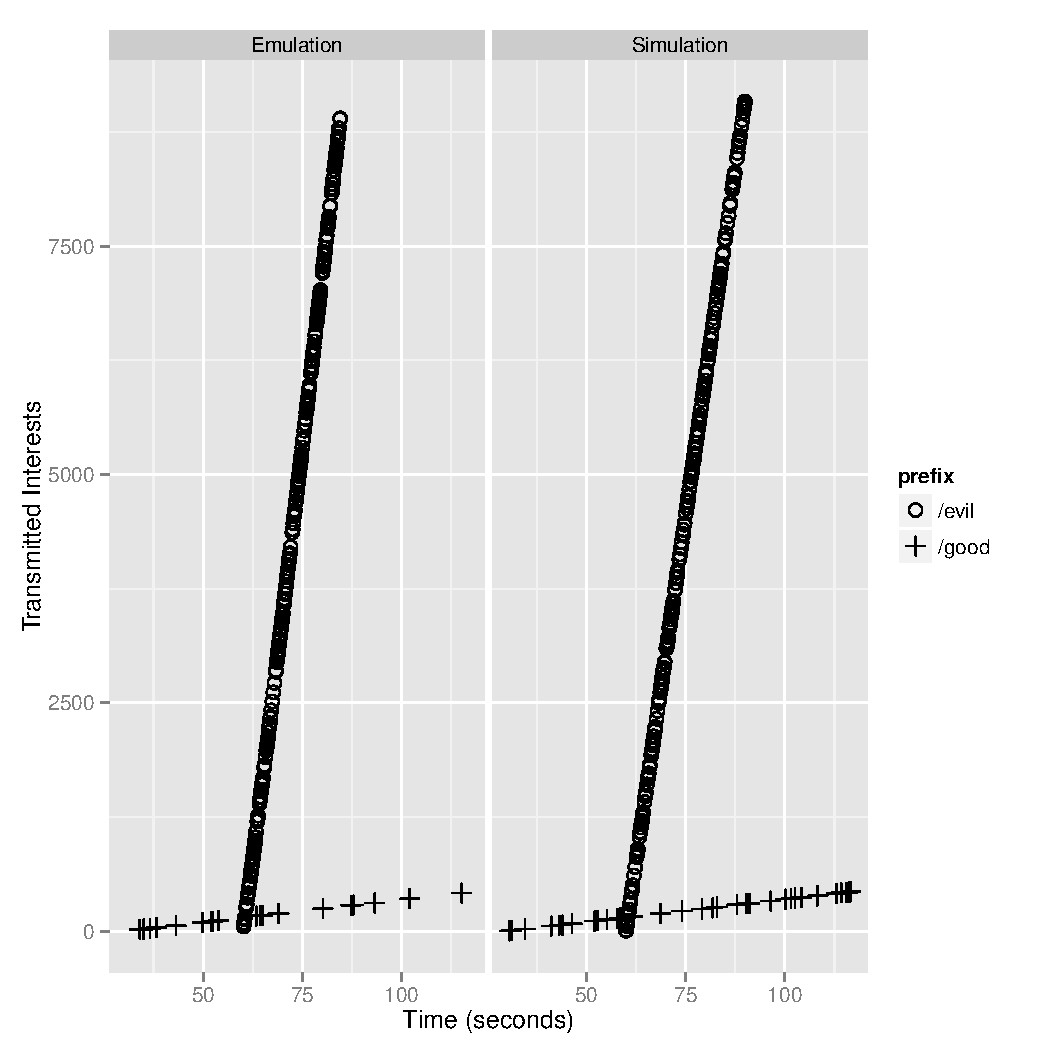
\includegraphics[scale=0.5]{figures/sim-emu-power.pdf}
  \caption{Strength of Interest flooding attack}
  \label{fig:simemupower}
\end{figure}

\begin{figure}[htpb]
  \centering
  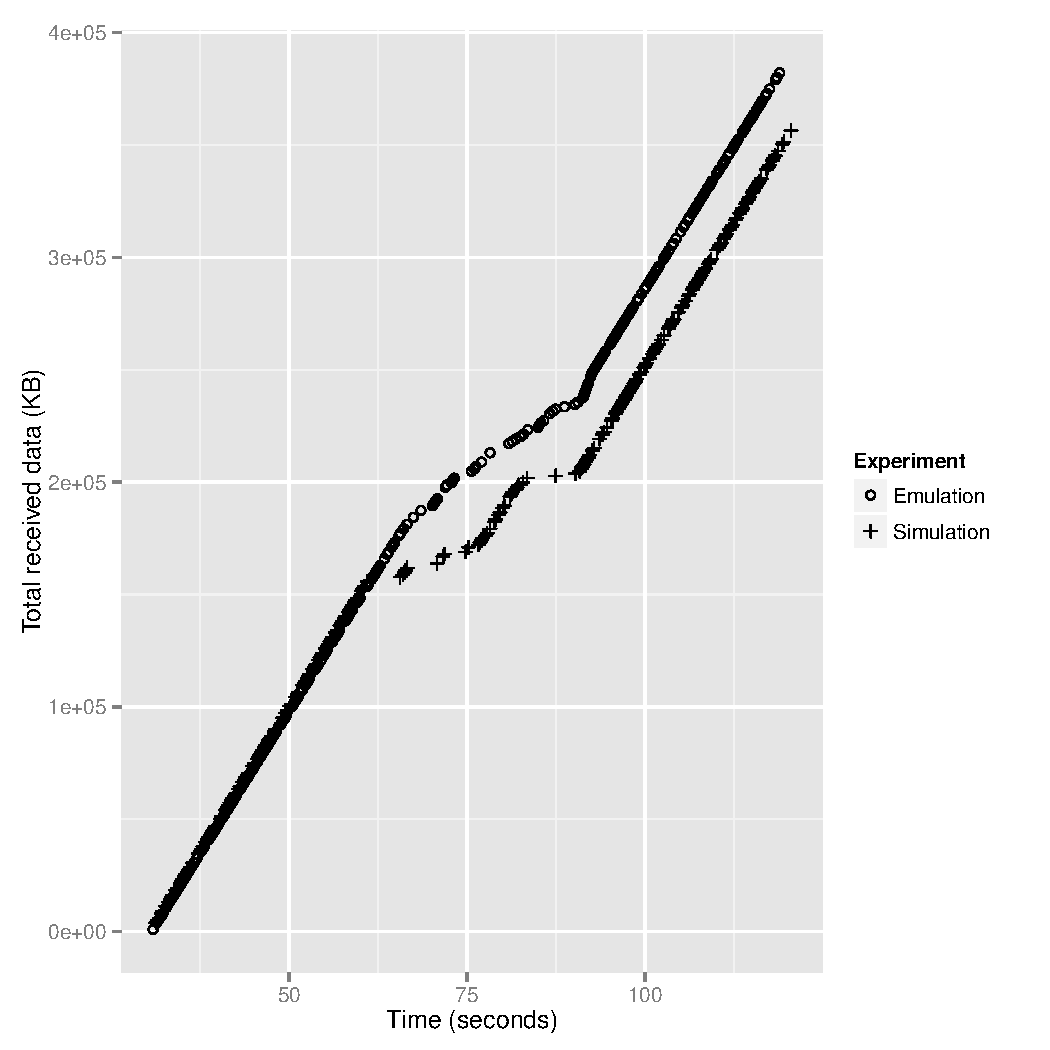
\includegraphics[scale=0.5]{figures/sim-emu-performance.pdf}
  \caption{Data retrieval by legitimate clients}
  \label{fig:simemuperf}
\end{figure}


